\section{Integração de Funções com Limites Infinitos ou Singularidades (Integrais Impróprias)}

\begin{enumerate}

\item
O integrando tem um limite finito nos limites de interpolação, mas não pode ser calculado nestes limites de integração. Por exemplo, \esp{\displaystyle \frac{\sin x}{x}} em \esp{x=0}:

\[
 \lim_{x \to 0} \, \frac{\sin x}{x} = 1 \, ; \qquad \displaystyle \frac{\sin (0)}{0} \mbox{ (singular)}
\]

\item
O limite superior é $+\infty$ ou o limite inferior é $-\infty$.

\item
Tem uma singularidade integrável em qualquer um dos limites. Por exemplo, \esp{x^{1/2}} em \esp{x=0}

\[
 \begin{array}{ll}
  \displaystyle \int_0^1 \, x^{-1/2} \, dx & = \displaystyle \lim_{h \to 0} \, \int_h^1 \, x^{-1/2} \, dx = \lim_{h \to 0} \, \left. \displaystyle \frac{x^{1/2}}{1/2} \right|_h^1 = \lim_{h \to 0} \, (2\,\sqrt{1} - 2\,\sqrt{h}) \\
  & = 2\,\sqrt{1} = 2
 \end{array}
\]

\item
Tem uma singularidade integrável em um ponto conhecido ou desconhecido entre os limites da integração.

\begin{description}

\item
\textbf{Integral Tipo 1}:

\begin{equation}
 \label{cap2:sec8:eq1}
 I = \int_{-\infty}^\infty exp\,(-x^2)\,dx \qquad \mbox{(caso b)}
\end{equation}

\item
\textbf{Integral Tipo 2}: 

\begin{equation}
 \label{cap2:sec8:eq2}
 I = \int_0^1 \frac{1}{\sqrt{x}\,(e^x + 1)} \, dx
\end{equation}

\begin{itemize}
\item 
O integrando é singular em $x = 0$ ($f(x) \rightarrow \infty$ para $x \rightarrow 0$)
\end{itemize}

\item
\textbf{Integral Tipo 3}:

\begin{equation}
 \label{cap2:sec8:eq3}
 I = \int_0^1 x^{0.7} \, \cos\,(x) \, dx
\end{equation}

\begin{itemize}
\item 
A função (integrando) não é analítica em $x = 0$.
\end{itemize}

\end{description}

\end{enumerate}

\subsection{Tipo 1}

\[
 I = \int_{-\infty}^\infty \, f\,(x) \, dx
 \quad \mbox{ou} \quad
 I = \int_{-\infty}^b \, f\,(x) \, dx
 \quad \mbox{ou} \quad
 I = \int_a^\infty \, f\,(x) \, dx
\]

\textbf{OBS1:} Uma função que é integrável em um domínio infinito ou semi-infinito é aproximadamente zero exceto em uma ?curta? parte do domínio. Por exemplo,

\[
 I = \int_{-\infty}^\infty \, e^{-x^2} \, dx
\]

\begin{figure}[htb]
 \centering
 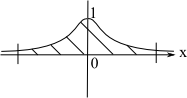
\includegraphics[scale=1.0]{capitulos/capitulo2/figuras/int_func_lim_inf1.png}
 \caption{?}
 \label{fig:int_func_lim_inf1}
\end{figure}

\textbf{OBS2:} Se $f(x)$ for analítica em $[-\infty,\infty]$, o método mais eficiente para a integração numérica é a regra do trapézio estendida.

\[
 I = h \, \sum_{i=-M}^M \, f\,(x_i)
\]

\begin{figure}[htp]
 \centering
 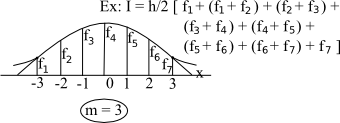
\includegraphics[scale=1.0]{capitulos/capitulo2/figuras/int_func_lim_inf2.png}
 \caption{?}
 \label{fig:int_func_lim_inf2}
\end{figure}

onde $x_{i} = i \ast h$ e $M$ é um inteiro tal que $\infty$ seja aproximado por $M \ast h$.

\begin{example}
 \esp{I = \displaystyle \frac{1}{\sqrt{\pi}} \, \int_{-\infty}^\infty \, e^{-x^2}} com 20, 40 e 80 intervalos

\textbf{Solução:} \esp{I \approx \displaystyle \frac{1}{\sqrt{\pi}} \, \int_{-10}^{10} \, e^{-x^2}}

\[N = 20 \rightarrow I = 1.000104\]
\[N = 40 \rightarrow I = 1.000001\]
\[N = 80 \rightarrow I = 1.000000\]

Valor exato: $I = 1.000000$
\end{example}

\subsection{Tipo 2}

\[
 I = \int_a^b \, f\,(x) \, dx
\]

onde $a$ e $b$ são finitos, mas $f(x)$ é singular em $a$, $b$ ou ambos.

\begin{enumerate}

\item 
Transformar $[a,b]$ em $[+\infty,-\infty]$ através de mudança de coordenadas.

\item
Aplicar regra do trapézio estendida

\end{enumerate}

\textbf{Mudança de coordenadas}

\[
 \begin{array}{l}
 \xi \qquad \xi\,(?)
 \left\{
 \begin{array}{l}
  \xi\,(a) = - \infty \\
  \xi\,(b) = + \infty
 \end{array}
 \right. \\
 x = x\,(\xi)
 \end{array}
\]

\begin{equation}
 \label{cap2:sec8:eq1}
 I = \int_a^b \, f\,(x) \, dx = \int_{-\infty}^\infty \, f\,(x\,(\xi)) \, \left( \frac{dx}{d\xi} \right) \, dx
\end{equation}

\underline{\textbf{Transformação Exponencial:}}

\begin{equation}
 \label{cap2:sec8:eq2}
 x\,(\xi) = \frac{1}{2} \left[ a + b + (b - a) \, tanh\,(\xi) \right]
\end{equation}

onde

\begin{equation}
 \label{cap2:sec8:eq3}
 tanh\,(\xi) = \frac{e^\xi - e^{-\xi}}{e^\xi + e^{-\xi}}
\end{equation}

\begin{figure}[htb]
 \centering
 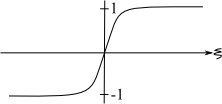
\includegraphics[scale=1.0]{capitulos/capitulo2/figuras/int_func_lim_inf3.png}
 \caption{?}
 \label{fig:int_func_lim_inf3}
\end{figure}

Para

\[
 \begin{array}{l}
  \xi = + \infty \Rightarrow tanh\,(+\infty) = 1 \Rightarrow x\,(+\infty) = b \\
  \xi = - \infty \Rightarrow tanh\,(-\infty) = -1 \Rightarrow x\,(-\infty) = a
 \end{array}
\]

\begin{equation}
 \label{cap2:sec8:eq4}
 \xi\,(x) = tanh^{-1} \left( \frac{2\,x - a - b}{b - a} \right)\,, \qquad x \in [a,\,b]
\end{equation}

\textbf{OBS1:} Para $\xi = 2.64665 \Rightarrow tanh = 0.99 \Rightarrow x \approx b$

\[
 ?
\]

\textbf{OBS2:} A precisão da integração é função da escolha da transformação.\\

\underline{\textbf{Dupla Exponenciação}}

\begin{equation}
 \label{cap2:sec8:eq5}
 \xi\,(x) = \frac{1}{2} \, \left[ a + b + (b - a) \, tanh \, \left( \frac{\pi}{2} \, sinh\,(\xi) \right) \right]
\end{equation}

\begin{equation}
 \label{cap2:sec8:eq6}
 sinh\,(\xi) = \frac{e^\xi - e^{-\xi}}{2}
\end{equation}

\begin{equation}
 \label{cap2:sec8:eq7}
 cosh\,(\xi) = \frac{e^\xi + e^{-\xi}}{2}
\end{equation}

\begin{equation}
 \label{cap2:sec8:eq8}
 \frac{dx}{d\xi} = \frac{(b-a) \, \displaystyle \frac{\pi}{4} \, cosh(\xi)}{cosh^2 \, \left[ \displaystyle \frac{\pi}{2} \, sinh\,(\xi) \right]}
\end{equation}

Eq. \ref{cap2:sec8:eq5} e \ref{cap2:sec8:eq8} $\rightarrow$ \ref{cap2:sec8:eq1}

\begin{equation}
 \label{cap2:sec8:eq9}
 I = h \, \sum_{k=-N}^N \, f\,(x_k) \, \left( \frac{dx}{d\xi} \right)_k
\end{equation}

onde

\[\xi_{k} = k \ast h\]

(h é predefinido)\\

\textbf{OBS:} Quão grande deve ser $N$?\\

Quando \esp{\xi_{k}} cresce \esp{\Rightarrow cosh^2 \, \left[ \displaystyle \frac{\pi}{2}\,sinh\,(\xi_k) \right] \rightarrow \displaystyle \frac{1}{4} \, exp\,\left[ \frac{\pi}{2} \, exp\,(\xi) \right]}, ou seja, o denominador de $ \displaystyle \frac{dx}{d\xi}$ cresce duplo-exponencialmente podendo causar \textit{overflow}.

Por exemplo,

\[
 \begin{array}{ll}
  & \displaystyle \frac{1}{4} \, exp\,\left[ \frac{\pi}{2} \, exp\,(\xi_k) \right] \approx \underbrace{2 \, \cdot \, 10^{38}}_{\footnotesize{\mbox{máximo número}}} \\
  \Rightarrow & \xi_k \approx 4 \Rightarrow N\,h < 4 \\
  & \\
  & \xi \approx 6.1 \Rightarrow f\,(\xi) \approx 3.6 \, \cdot \, 10^{303}
 \end{array}
\]

Outro exemplo é:

\[
  I = \int_0^2 \sqrt{1 + \frac{1}{x}} \, dx \qquad
 \begin{array}{l}
  a = 0 \\
  b = 2
 \end{array}
\]

Em \esp{x = 0}, \esp{\sqrt{1 + \displaystyle \frac{1}{x}}} é singular.\\

\underline{\textbf{Transformações de Coordenadas}}

\begin{equation}
 \label{cap2:sec8:eq10}
 \begin{array}{ll}
  x_k & = \displaystyle \frac{1}{2} \left[ 0 + 2 + (2 - 0) \, tanh \, \left( \frac{\pi}{2} \, sinh\,(\xi) \right) \right] \vspace*{0.2cm} \\
  x_k & = \displaystyle \frac{1}{2} \left[ 2 + 2 \, tanh \, \left( \frac{\pi}{2} \, sinh\,(\xi_k) \right) \right] \vspace*{0.2cm} \\
      & = 1 + tanh \, \left( \displaystyle \frac{\pi}{2} sinh\,(\xi_k) \right)
 \end{array}
\end{equation}

Substituindo em (a) e adotando os limites de $\xi$ [-4, 4]

{
%\begin{table}[htp]
\footnotesize
	\begin{center}
		\begin{tabular}{|c|c|c|}
		\hline		
		\textbf{N} & \textbf{I} \\
		\hline \hline
		10 & 3.600710 \\
		\hline
		20 & 3.595706 \\
		\hline
		30 & 3.595706 \\
		\hline
		\end{tabular}
	\end{center}
	\label{cap2:sec6:tab3}
%\end{table}
}